\documentclass[aspectratio=169]{beamer}
%=======================
%       IMPORTANT
%=======================

% This document is meant to be compiled with
% LuaLaTeX and the -shell-escape option.
% The "svg" package also requires Inkscape to
% be on the path.

%=======================
%       IMPORTS
%=======================

\usepackage{amsmath, amsthm, amssymb}   % Math symbols, environments etc.
\usepackage{fontspec}                   % For Unicode fonts
\usepackage{unicode-math}               % For Unicode math fonts
\usepackage{microtype}                  % Nicer interword spacing
\usepackage{polyglossia}                % Provides locale-specific formatting
\usepackage{csquotes}
\usepackage{caption}                    % Provides captions outside of floats
\usepackage{svg}                        % For including SVG files
\usepackage{booktabs}                   % Nicer tables
\usepackage{tabularx}                   % Allows for linebreaks in tables

\usepackage{tikz}
\usetikzlibrary{positioning}

\usepackage{pgfplots}
\pgfplotsset{compat=newest}
\usepackage{pgfplotstable}
\usepackage{pgf-pie}

\usepackage[
    backend = biber,
    style = ieee-alphabetic
]{biblatex}

%=======================
%     PACKAGE SETUPS
%=======================

% Set beamer theme
\usetheme{metropolis}
% \beamertemplatenavigationsymbolsempty
\metroset
{
    sectionpage = simple,
    subsectionpage = simple
}

% Use uppercase roman numerals for continuation
\makeatletter
\setbeamertemplate{frametitle continuation}{%
\usebeamerfont{frametitle}
(\@Roman\insertcontinuationcount)
}
\makeatother

% Custom description environment (https://tex.stackexchange.com/a/52299/176658)
\makeatletter
\def\Ldescription{%
  \@ifnextchar[{\beamer@testforospec}{\beamer@descdefault\beamer@descriptionwidth\@@Ldescription}%
}

\def\beamer@testforospec[{\@ifnextchar<{\beamer@scandefaultospec[}{\@Ldescription[}}%

\def\beamer@scandefaultospec[#1]{\def\beamer@defaultospec{#1}\Ldescription}

\def\@Ldescription[#1]{%
\setbox\beamer@tempbox=\hbox{\def\insertdescriptionitem{#1}
  \usebeamertemplate**{description item}}%
\beamer@descdefault\wd\beamer@tempbox\@@description%
}%

\def\@@Ldescription{%
  \beamer@descdefault35pt%
  \list
  {}
  {\labelwidth\beamer@descdefault\leftmargin2.8em\let\makelabel\beamer@Ldescriptionitem}%
  \beamer@cramped%
  \raggedright
  \beamer@firstlineitemizeunskip%
}

\def\endLdescription{\ifhmode\unskip\fi\endlist}
\long\def\beamer@Ldescriptionitem#1{%
  \def\insertdescriptionitem{#1}%
  \hspace\labelsep{\parbox[b]{\dimexpr\textwidth-\labelsep\relax}{%
        \usebeamertemplate**{description item}%
    }}}
\makeatother

% Font settings
\setmonofont[Scale=0.8]{Fira Mono}

\setmathfont{TeX Gyre Pagella Math}

% Captions
\captionsetup{justification=centering}

% Language Setup
\setdefaultlanguage{english}
\setotherlanguage[spelling=new, babelshorthands=true]{german}

% Set path for graphics
\graphicspath{{./graphics/}}

% TikZ
\tikzstyle{server} = [
    rectangle,
    draw,
    fill = gray!20,
    text centered,
    rounded corners,
    minimum width = 4.5cm,
    minimum height = 1cm
]

\tikzstyle{os} = [
    rectangle,
    draw,
    fill = blue!20,
    text centered,
    rounded corners,
    minimum width = 4.5cm,
    minimum height = 1cm
]

\tikzstyle{vmm} = [
    rectangle,
    draw, fill = orange!40,
    text centered,
    rounded corners,
    minimum width = 10.25cm,
    minimum height = 1cm
]

\tikzstyle{app} = [
    rectangle,
    draw,
    fill = green!20,
    text centered,
    rounded corners,
    minimum width = 1cm
]

% BibLaTeX
\addbibresource{{../green.bib}}
\addbibresource{{../pictures.bib}}

% hyperref setup
\hypersetup
{
    pdfencoding = auto      % For umlauts in PDF sections
}

%=======================
%    CUSTOM COMMANDS
%=======================

% Math commands
\newcommand{\tat}{\textasciitilde{} }

% Command to center a single cell in a tabular
\newcommand{\cc}[1]{\multicolumn{1}{c}{#1}}

%=======================
%  DOCUMENT INFORMATION
%=======================

\title{Server Consolidation in \\ Virtualized Data Centers}
\subtitle{Seminar \textit{Green Networking}}
\author[L.~Richardt]{Leon Richardt}
\date[2020-01-10]{10 January 2020}
\institute{Osnabrück University}

\begin{document}

\begin{frame}
    \titlepage
\end{frame}

\begin{frame}{Table of Contents}
    \tableofcontents
\end{frame}

\section{Principles}
\subsection{Power Consumption in Data Centers}

%### FRAME ###

\begin{frame}{\insertsectionhead: \insertsubsectionhead}
    \begin{columns}
        \begin{column}{0.5\paperwidth}
            \begin{figure}
                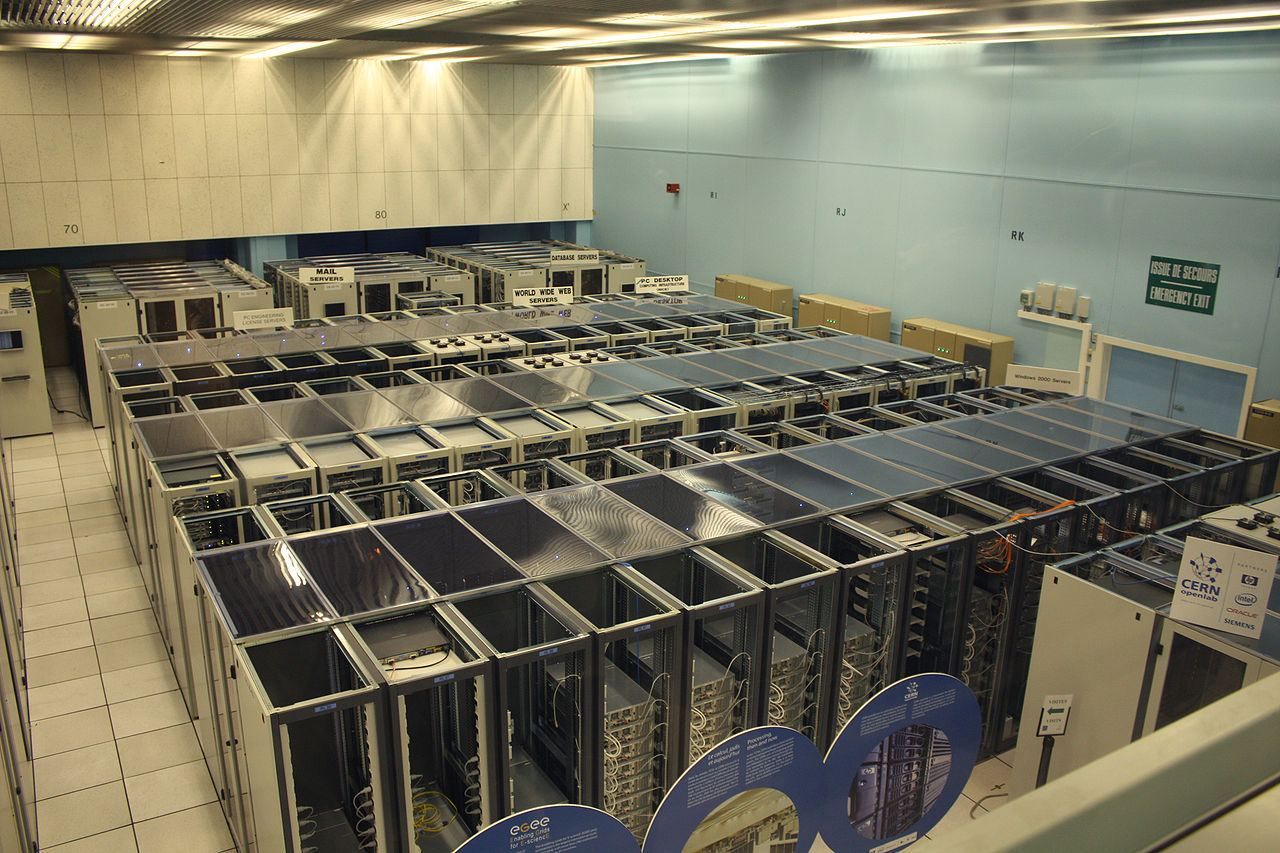
\includegraphics[width = 0.8\columnwidth, keepaspectratio]{cern_data_center}
                \caption{Server racks at CERN \cite{cern_data_center}}
            \end{figure}
        \end{column}

        \begin{column}{0.5\paperwidth}
            \begin{figure}
                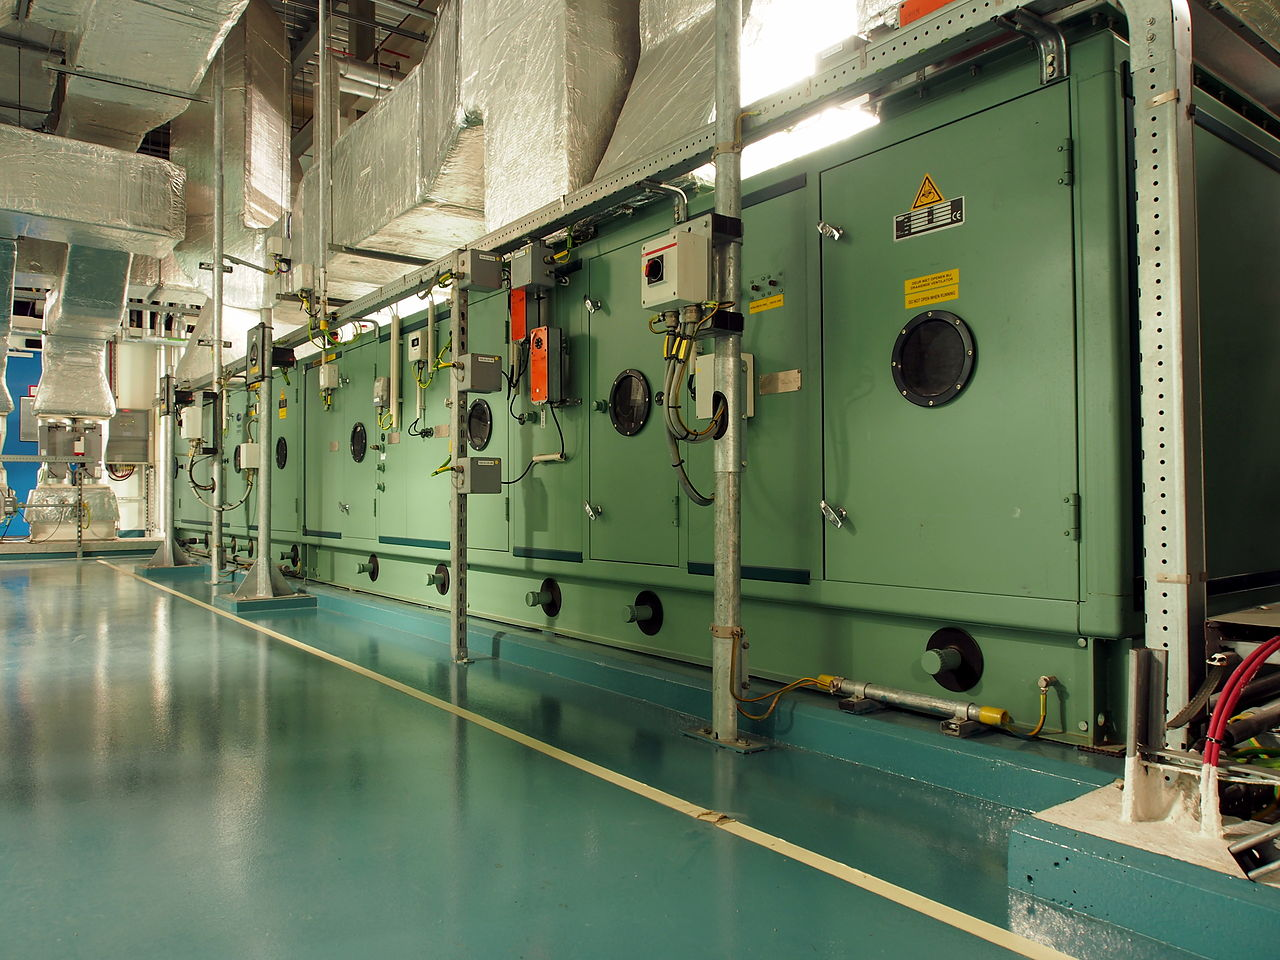
\includegraphics[width = 0.8\columnwidth, keepaspectratio]{hvac}
                \caption{Ventilation unit \cite{hvac}}
            \end{figure}
        \end{column}
    \end{columns}
\end{frame}

%### FRAME ###

\begin{frame}{\insertsectionhead: \insertsubsectionhead}
    \begin{columns}
        \begin{column}{0.5\paperwidth}
            \begin{figure}
                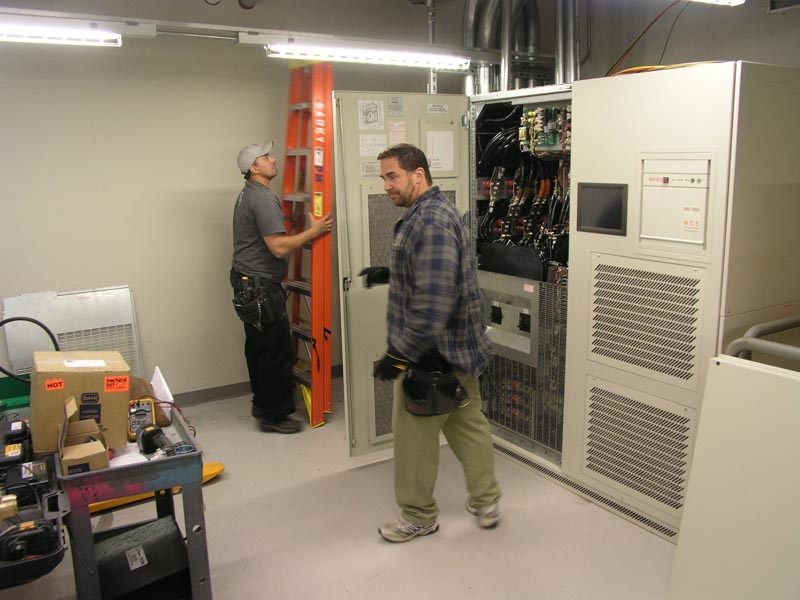
\includegraphics[width = 0.8\columnwidth, keepaspectratio]{ups}
                \caption{UPS in a data center \cite{ups}}
            \end{figure}
        \end{column}

        \begin{column}{0.5\paperwidth}
            \begin{figure}
                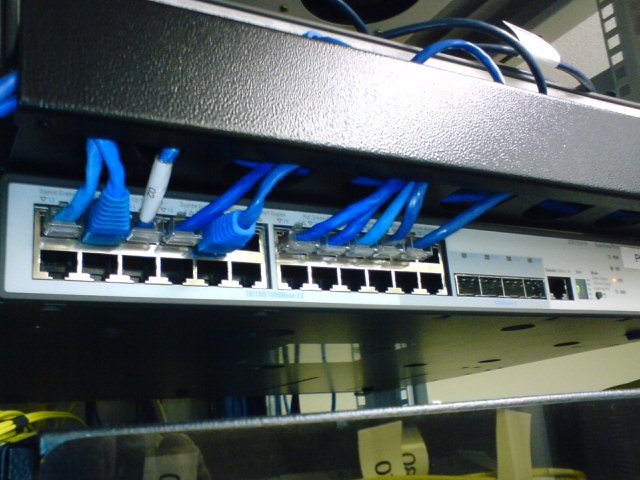
\includegraphics[width = 0.8\columnwidth, keepaspectratio]{network_switch}
                \caption{Network switch \cite{network_switch}}
            \end{figure}
        \end{column}
    \end{columns}
\end{frame}

%### FRAME ###

\begin{frame}{\insertsectionhead: \insertsubsectionhead}
    \begin{figure}
        \centering
        \resizebox{0.8\paperwidth}{!}{%
            \begin{tikzpicture}
                \pie[
                    radius = 3,
                    text = legend,
                    explode = {0, 0, 0, 2, 2, 0.1, 0.1}
                ]
                {
                    40/{Server Hardware},
                    5/{Storage Devices},
                    5/{Network Devices},
                    1/{Lighting},
                    2/{Transformer Overhead},
                    9/{UPS Overhead},
                    38/{Cooling Equipment}
                }
            \end{tikzpicture}%
        }

        \caption{Average distribution of power consumption by different data center components, see \cite{masanet_estimating_2011}.}
    \end{figure}
\end{frame}

%### FRAME ###

\begin{frame}{\insertsectionhead: \insertsubsectionhead}
    Common features of data center workloads:

    \begin{tabularx}{\textwidth}{rX}
        \textbf{High Idle Times} & Average server utilization is between 10\% and 50\% for 80\% of the time\footcite{barroso_epc_2007}. \\
        \textbf{Bursty Workloads} & Server load often occurs in bursts\footcite{varasteh_survey_2017}. \\
        \textbf{Periodicity} & For some use cases (e.g.\ streaming services), workloads may occur with periodic patterns. \\
    % TODO: add more here
    \end{tabularx}
    % \end{description}
\end{frame}
\subsection{Virtual Machines}

% ### FRAME ###

\begin{frame}{\insertsectionhead: \insertsubsectionhead}
    Terminology:
    \begin{description}
        \item [VM] virtual machine
        \item [VMM] virtual machine monitor
        \item [PM] physical machine
        \item [SLA] service-level agreement
    \end{description}
\end{frame}

% ### FRAME ###

\begin{frame}{\insertsectionhead: \insertsubsectionhead}
    \begin{itemize}
        \item
            VMs represent \enquote{an efficient, isolated duplicate of the real machine}\footcite{popek_vm_1974}.

        \item
            For our purposes: VM \(\approx\) OS + Applications.

        \item
            VMMs provision and manage CPU/memory/device allocation of VMs.

        \item
            VMs can be moved between physical machines without losing their state.
    \end{itemize}
\end{frame}

% ### FRAME ###

\begin{frame}{\insertsectionhead: \insertsubsectionhead}
    \begin{figure}
        \resizebox{0.9\paperwidth}{!}{%
            \hspace{-0.95cm}
            \begin{tikzpicture}

                % PM 1
                \node [server] (pm1) {PM \(P_1\)};
                \node [os, above = 0.2cm of pm1] (os1) {OS \(O_1\)};
                \node [above = 0.3cm of os1.north] (dotsApp1) {\dots};
                \node [app, left = 0.1cm of dotsApp1] (app11) {App \(A_{1,1}\)};
                \node [app, right = 0.1cm of dotsApp1] (app1k) {App \(A_{1,k}\)};

                % PM 2
                \node [server, right = of pm1] (pm2) {PM \(P_2\)};
                \node [os, above = 0.2cm of pm2] (os2) {OS \(O_2\)};
                \node [above = 0.3cm of os2.north] (dotsApp2) {\dots};
                \node [app, left = 0.1cm of dotsApp2] (app21) {App \(A_{2,1}\)};
                \node [app, right = 0.1cm of dotsApp2] (app2l) {App \(A_{2,l}\)};

                \node [right = of pm2] (dotsPm) {\dots};

                % PM n
                \node [server, right = of dotsPm] (pmN) {PM \(P_n\)};
                \node [os, above = 0.2cm of pmN] (osN) {OS \(O_n\)};
                \node [above = 0.3cm of osN.north] (dotsAppN) {\dots};
                \node [app, left = 0.1cm of dotsAppN] (appN1) {App \(A_{n,1}\)};
                \node [app, right = 0.1cm of dotsAppN] (appNm) {App \(A_{n,m}\)};

            \end{tikzpicture}%
        }% end \resizebox
    \caption{Data center architecture without virtualization}
    \end{figure}

    \begin{itemize}
        \item [\(\implies\)]<2->
            All servers must be running to support SLAs, even when current demand for a particular application is low.

        \item [\(\implies\)]<2->
            Some programs may require a specific architecture (e.g.\ x86, ARM) or specific OS (e.g.\ Linux, Windows).
            This may lead to fragmentation.
    \end{itemize}
\end{frame}

% ### FRAME ###

\begin{frame}{\insertsectionhead: \insertsubsectionhead}
    \begin{figure}
        \resizebox{!}{0.75\paperheight}{
            \begin{tikzpicture}

                % PM 1
                \node [server, minimum width = 10.25cm] (pm1) {PM \(P_1\)};
                \node [vmm, above = 0.2cm of pm1] (vmm1) {VMM \(V_1\)};

                \node [above = 0.5cm of vmm1] (dotsOs1) {\dots};

                % OS 1,1
                \node [os, left = 0.3cm of dotsOs1] (os11) {OS \(O_{1,1}\)};
                \node [above = 0.3cm of os11.north] (dotsApp1) {\dots};
                \node [app, left = 0.1cm of dotsApp1] (app111) {App \(A_{1,1,1}\)};
                \node [app, right = 0.1cm of dotsApp1] (app11i) {App \(A_{1,1,i}\)};

                % OS 1,\alpha
                \node [os, right = 0.3cm of dotsOs1] (os1Alpha) {OS \(O_{1,\alpha}\)};
                \node [above = 0.3cm of os1Alpha.north] (dotsAppAlpha) {\dots};
                \node [app, left = 0.1cm of dotsAppAlpha] (appAlpha11) {App \(A_{1,\alpha,1}\)};
                \node [app, right = 0.1cm of dotsAppAlpha] (appAlpha1J) {App \(A_{1,\alpha,j}\)};

                \node [below = 0.3cm of pm1] (dotsPm) {\(\vdots\)};

                % PM n
                \node [below = 1.5cm of dotsPm] (dotsOsN) {\dots};

                % OS n,1
                \node [os, left = 0.3cm of dotsOsN] (osN1) {OS \(O_{n,1}\)};
                \node [above = 0.3cm of osN1] (dotsAppN1) {\dots};
                \node [app, left = 0.1cm of dotsAppN1] (appN11) {App \(A_{n,1,1}\)};
                \node [app, right = 0.1cm of dotsAppN1] (appN1K) {App \(A_{n,1,k}\)};

                % OS n,\beta
                \node [os, right = 0.3cm of dotsOsN] (osNBeta) {OS \(O_{n,\beta}\)};
                \node [above = 0.3cm of osNBeta] (dotsAppNBeta) {\dots};
                \node [app, left = 0.1cm of dotsAppNBeta] (appNBeta1) {App \(A_{n,\beta,1}\)};
                \node [app, right = 0.1cm of dotsAppNBeta] (appNBetaL) {App \(A_{n,\beta,l}\)};

                \node [vmm, below = 0.5cm of dotsOsN] (vmmN) {VMM \(V_n\)};
                \node [server, below = 0.2cm of vmmN, minimum width = 10.25cm] (pmN) {PM \(P_n\)};

            \end{tikzpicture}%
        }% end \resizebox
    \caption{Data center architecture using virtualization}
    \end{figure}
\end{frame}

% ### FRAME ###

\begin{frame}{\insertsectionhead: \insertsubsectionhead}
    \begin{itemize}
        \item [\(\implies\)]
            Enables usage of uniform host platform (e.g.\ only CentOS servers running on x86).

        \item [\(\implies\)]
            VMs can be moved between PMs to minimize the number of active PMs: \alert{energy savings}.

        \item [\(\implies\)]
            VMs can be provisioned on demand: \alert{scalability}.
    \end{itemize}
\end{frame}

\section{Optimization Approaches}

% ### FRAME ###

\begin{frame}{\insertsectionhead}
    \centering
    \large
    What criteria can we consider when deciding which VMs to migrate?
\end{frame}


\subsection{Hardware Utilization}

% ### FRAME ###

\begin{frame}{\insertsectionhead: \insertsubsectionhead}
    \begin{itemize}
        \item
            CPU and memory utilization describe the load observed on a PM.

        \item
            High CPU/memory load on a single PM \(\implies\) data center is \alert{overloaded}.

        \item
            Low CPU/memory load over the whole system \(\implies\) data center is \alert{underloaded}.
    \end{itemize}

    \vfill
    \centering
    \textbf{Idea}: Migrate VMs whenever the system is under- or overloaded.
\end{frame}

% ### FRAME ###

\begin{frame}{\insertsectionhead: \insertsubsectionhead}
    \begin{Ldescription}
        \item [Reactive Policy \textnormal{(Migration Controller, \textit{MC})}]
            Rebalancing is done immediately when a threshold violation is detected.

            On an overloaded PM, a VM is determined for migration to the least loaded PM capable of hosting the VM.
            If no such PM exists, a new server may be booted.

            In an underload situation, the VMs on the least loaded PM are transferred to other PMs.
    \end{Ldescription}
\end{frame}

% ### FRAME ###

\begin{frame}{\insertsectionhead: \insertsubsectionhead}
    \begin{Ldescription}
        \item [Proactive Policy \textnormal{(Workload Placement Controller, \textit{WP})}]
            Rebalancing is done in predetermined intervals.

            Historical data (resource utilization traces) are used to determine how much capacity is provisioned during each interval.
            During an interval, no additional VMs will be started, and no existing VMs will be stopped.
    \end{Ldescription}
\end{frame}

% ### FRAME ###

\begin{frame}{\insertsectionhead: \insertsubsectionhead}
    \begin{Ldescription}
        \item [Mixed Policies]
            Historical data is used to predict the expected workload profile in the next interval.

            When violations occur during an interval, the same migration strategy as above is used.
            In another variation, historical data is considered for rebalancing on every threshold violation.
    \end{Ldescription}
\end{frame}

% ### FRAME ###

\begin{frame}{\insertsectionhead: \insertsubsectionhead}
    \centering
    \begin{figure}
        \resizebox{0.8\paperwidth}{!}{\includesvg{reactive_proactive}}
        \caption{Performance of different provisioning policies \cite{gmach_resource_2009}}
    \end{figure}
\end{frame}

\subsection{Network Traffic}

\begin{frame}{\insertsectionhead: \insertsubsectionhead}
    \begin{itemize}
        \item
            Many modern data center applications communicate over the network.

        \item
            Cost of communication differs based on network placement of VMs.

        \item
            Cost of communication also depends on the rate of communication between VMs.
    \end{itemize}

    \vfill
    \centering
    \textbf{Idea}: Place VMs such that total communication cost is minimized.
\end{frame}

\begin{frame}{\insertsectionhead: \insertsubsectionhead}
    \begin{tabular}{rl}
        \(v_1, \dots, v_n\) & VMs \\
        \(s_1, \dots, s_n\) & Slots (a slot represents the ability to place a VM on a PM) \\
        \(C_{ij}\) & Communication cost between slots \(s_i\) and \(s_j\) \\
        \(D_{ij}\) & Traffic rate between VMs \(v_i\) and \(v_j\) \\
        \(g_i\) & External communication cost of slot \(s_i\) \\
        \(e_i\) & External traffic rate of VM \(v_i\)
    \end{tabular}

    \uncover<2->{%
    \vfill
    \centering
    \textbf{Goal}: Find a VM-to-slot mapping \(\pi \colon [1, \dots, n] \to \, [1, \dots, n]\) that minimizes
    \[
        \sum_{i, j = 1, \dots, n} D_{ij} C_{\pi(i) \pi(j)}
        + \sum_{i = 1}^{n} e_i g_{\pi(i)}.
    \]%
    }
\end{frame}

\begin{frame}{\insertsectionhead: \insertsubsectionhead}
    \begin{itemize}
        \item
            Unfortunately, finding an optimal \(\pi\) is NP-hard\footcite{meng_traffic_aware_2010}.

        \item
            \(O(n^4)\) approximation algorithm:

            \begin{enumerate}
                \item
                    Cluster slots such that slots with low intercommunication rate are close to each other.

                \item
                    Cluster VMs such that VMs with high intercommunication traffic are close to each other.
                    Ensure clusters have the same size.

                \item
                    Recursively map slot clusters to VM clusters.
            \end{enumerate}
    \end{itemize}
\end{frame}

\begin{frame}{\insertsectionhead: \insertsubsectionhead}
    \centering
    \begin{table}
        \begin{tabular}{cccc}
            \textbf{Topology} & \textbf{Algorithm} & \textbf{Objective Function} & \textbf{CPU time} \\ \toprule
                              & LOPI               & 0.9732                      & 22 \\
            VL2               & SA                 & 1.0000                      & 27 \\
                              & Cluster-and-Cut    & 0.9375                      & 11 \\ \midrule
                              & LOPI               & 1.0000                      & 29 \\
            BCube             & SA                 & 0.9860                      & 35 \\
                              & Cluster-and-Cut    & 0.8462                      & 14 \\ \bottomrule
        \end{tabular}

        {\footnotesize (Note: Objective function value has been normalized to 1.)}

        \vspace{0.5cm}
        \caption{
            Comparison of different approximation algorithms on different network topologies.
            The data is obtained from trace-driven simulations. \cite{meng_traffic_aware_2010}
        }
    \end{table}
\end{frame}

\begin{frame}{\insertsectionhead: \insertsubsectionhead}
    \begin{itemize}
        \item [\(\implies\)]
            Effectiveness depends on the underlying network topology.

        \item [\(\implies\)]
            Only \enquote{sensibly} applicable when many VMs inside the same data center need to communicate with each other.

        \item [\(\implies\)]
            Slightly better objective function value when compared to other approximations.
            On \enquote{favorable} network topologies, the improvement can range up to 15\%.

        \item [\(\implies\)]
            \dots{} but twice as fast!
    \end{itemize}
\end{frame}

\section{Evaluation}

\begin{frame}{\insertsectionhead}
    \begin{Ldescription}
        \item [Applicability]
            Not every optimization approach may be applicable (or effective) in every data center.

            For example, Cluster-and-Cut can only reasonably be used as the dominant placement strategy when VMs inside the same facility show high intercommunication rates.
            (Probably not the case for consumer-oriented cloud computing providers but may very well be true for enterprise-oriented solutions.)
            Some strategies, however, (e.g.\ temperature-optimizing) may be more generally applicable.
    \end{Ldescription}
\end{frame}

\begin{frame}{\insertsectionhead}
    \begin{Ldescription}
        \item [Experimental Data]
            \enquote{New} migration/placement strategies are usually only simulated on traces of past data center workloads.
            Therefore, it is hard to evaluate how these strategies hold up under real-world conditions.

            This is understandable from a business standpoint:
            No one wants to put their service infrastructure at risk.
    \end{Ldescription}
\end{frame}

\begin{frame}{\insertsectionhead}
    \begin{Ldescription}
        \item [Balancing Optimization Aspects]
            It is unclear how to simultaneously pursue different optimization strategies.

            For example, a CPU utilization strategy may produce a contradicting VM placement to a network traffic strategy.
            Balancing those aspects likely requires a good understanding of the local conditions and workload profiles.
            This, in turn, means more work for the data center controllers.
    \end{Ldescription}
\end{frame}

\section{Conclusion \& Outlook}

\begin{frame}{\insertsectionhead}
    To summarize:

    \begin{itemize}
        \item
            Power consumption in data centers is influenced by a number of factors.

        \item
            Server consolidation by virtualization provides an effective tool for influencing these factors.
            Different strategies aim to optimize different factors.

        \item
            Placement strategies are not easy to compare with each other \textit{a priori}.
    \end{itemize}
\end{frame}

% #### FRAME ####

\begin{frame}{\insertsectionhead}
    \vspace{-0.8cm}
    \begin{figure}
        \pgfkeys{/pgf/number format/.cd,1000 sep={}}
        \begin{tikzpicture}
            \begin{axis}[
                width = 0.9\paperwidth,
                height = 0.85\paperheight,
                mlineplot,
                ymin = 0,
                ymax = 600,
                ytick = {0, 100, 200, 300, 400, 500, 600},
                xtick = data,
                xmajorgrids = false
            ]

                \addplot table {energy.dat};
                \addplot table {workloads.dat};
                \addplot table {traffic.dat};

                \legend{{Data Center Energy Usage}, {Data Center Workloads}, {Internet Traffic}};
            \end{axis}
        \end{tikzpicture}
        \caption{Projected relative data center energy usage \cite{iea_analysis_2019}}
    \end{figure}
\end{frame}

\begin{frame}{\insertsectionhead}
    In the future:

    \begin{itemize}
        \item
            As demand for computing power and more reliable online services increases, the field can be expected to stay and become even more relevant in the future.

        \item
            Even though Internet traffic will likely continue to grow, improvements in hardware and software are expected to offset increasing data center workloads.

        \item
            Containerization is becoming increasingly popular as an alternative to VMs.
    \end{itemize}
\end{frame}

\begin{frame}[standout]
    \huge Questions.
\end{frame}

% #### FRAME ####

\begin{frame}[allowframebreaks]{References}
    \printbibliography
\end{frame}
\end{document}
